
\documentclass{beamer}
\usepackage{pgfpages}
 %\setbeameroption{hide notes} % Only slides
%\setbeameroption{show only notes} % Only notes
\setbeameroption{show notes on second screen=right} % Both
\setbeamertemplate{note page}{\pagecolor{yellow!5}\insertnote}\usepackage{palatino}
% https://gist.github.com/andrejbauer/ac361549ac2186be0cdb

% \usetheme[hideothersubsections]{WrightState}
\usetheme[left,hideothersubsections,width=2cm]{WrightState} %2.5cm

\title{Data Mining Techniques and Mathematical Models for
the Optimal Scholarship Allocation Problem for a State University}
\author{Shuai Wang} %
\institute{Wright State University \\

	Department of Biomedical, Industrial \& Human Factors Engineering}
\date{December 6 2017}

\usepackage{natbib}  % for citation
\usepackage{comment}
\usepackage{geometry,array,graphicx,float,caption,subcaption,epstopdf,multiro
w}

% \usepackage{floatrow}
% \newfloatcommand{capbtabbox}{table}[][\FBwidth]

%https://tex.stackexchange.com/questions/193975/highlight-only-current
%-subsection-hide-subsections-of-other-sections

%https://tex.stackexchange.com/questions/193975/highlight-only-current
%-subsection-hide-subsections-of-other-sections

\setcounter{tocdepth}{1} % hide subsection in the table of content

\AtBeginSection[]{
% \ifnum \value{framenumber}>1
\begin{frame}<beamer>
%    \frametitle{Outline for section \thesection}
    \tableofcontents[currentsection]
  \end{frame}
}


\begin{comment}
\makeatletter
  \setbeamertemplate{sidebar \beamer@sidebarside}%{sidebar theme}
  {
    \beamer@tempdim=\beamer@sidebarwidth%
    \advance\beamer@tempdim by -6pt%
    \insertverticalnavigation{\beamer@sidebarwidth}%
    \vfill
    \ifx\beamer@sidebarside\beamer@lefttext%
    \else%
      \usebeamercolor{normal text}%
      \llap{\usebeamertemplate***{navigation symbols}\hskip0.1cm}%
      \vskip2pt%
    \fi%
}%
\makeatother
\end{comment}

% ------ begin ---------------------------------------

\begin{document}

%{% open a Local TeX Group
% \setbeamertemplate{sidebar}{}
\begin{frame}
        \titlepage
       
     \note[item]{Thank for attending my thesis defense.}
      \note[item]{My name is Shuai Wang, and I am from BIE department}
      \note[item]{my thesis topic is Data Mining Techniques and Mathematical Models for
      the Optimal Scholarship Allocation Problem for a State University}
\end{frame}
%}% end Local TeX Group


\begin{frame}
    \frametitle{Presentation Outline}
    
 \tableofcontents
 
\end{frame}


\section{Introduction}  

\subsection{Background}
\begin{frame}
    \frametitle{Background}
\begin{itemize}
\item In the United States, in the 2012-2013 academic year, there were a total 
of 20.4 million students in degree-granting institutions.
\item More than 80\% of them received financial aid and more than 70\% of
them received grants.
\item  Studies have shown that financial aid is one of the most important
factor in attracting student and is vital to enrollment marketing.
\end{itemize}
\note[item]{first,I'd like to talk about the background of the study}
\note[item]{For the school under study, nearly half of the revenue are from tuition income}
\end{frame}

\begin{frame}
	\frametitle{Background Cont.}
    Enrollment management consisted of approaches to help education institute
to meet the established goal such as:
   \begin{itemize}
   \item Attracting more high-caliber students.
   \item Diversify student body.
   \item Increase retention.
  % \item etc,.
   \end{itemize} 
   \note[item]{Enrollment management is critical part of university management}
   \note[item]{Typical enrollment management activity starts from reaching potential
   high school students and ends at graduation} 
\end{frame}



\begin{frame}
\frametitle{Background Cont.}
Financial aid is a critical part of enrollment management.
It helps the university:
\begin{itemize}
\item Providing more access to families who need help.
\item Stimulating more students to major in area having labor shortage.
\item Shaping and diversifying the student body.
\end{itemize}
\end{frame}



\subsection{Motivation}
\begin{frame}
\frametitle{Motivation}

\begin{enumerate}
\item \textbf{Non-optimal} usage of financial aid at university:

\begin{itemize}
\item   Over-spending financial aid budget would reduce revenue.
\item   Under-spending financial aid would potentially
undermine enrollment number and revenue. 
\end{itemize}

\item The tuition income account for nearly half on the 
yearly revenue.

\item The optimal allocation of scholarship problem has 
\textbf{not} been widely studied.

\end{enumerate}
\end{frame}

\subsection{Objective}
\begin{frame}  
    \frametitle{Objective}
The objectives of this study are:
\begin{enumerate}
    \item How does financial aid impact on student's
    decision?
\item What is the optimal scholarship for each student in favor of the over 
    all budget?
    \item How to optimally allocate the financial aid budget at school level?
\end{enumerate}

\end{frame}


%%%%%%%%%%%%%%%%%%%%%%
\subsection{Contribution}

\begin{frame}
    \frametitle{Contribution}
    \begin{itemize}
    \item Linking traditional prediction technique with optimization 
    technique to solve existing managerial problems  in the enrollment
    management such as:
    \begin{enumerate}
    \item Who should get more scholarship, by how much?
    \item What is the ideal overall financial budget for institute?
    \item Is it possible to give customized scholarship?
    \end{enumerate}
    
%     \item \textbf{A complete set of models} to
%     predict probability of enrollment, graduation
%     and number years of stay in terms of various scholarship
%     award.
%     \item \textbf{An optimization model} to determine the 
%     ideal scholarship level.
%     \item \textbf{Integration} of data mining techniques and 
%     optimization techniques.
    \end{itemize}
  
\end{frame}

\subsection{Results}


\begin{frame}
    \frametitle{Results example}
\begin{table}[H]
\centering
 \tiny
 \setlength\tabcolsep{3pt}
    \begin{tabular}{|c|c|c|c|c|c|c|c|c|c|c|c|}
    \hline \hline
    \multicolumn{12}{ |c| }{GPA 2.9, ACT 19 }  \\ \hline
& Student               & 0       & 1000    & 2000    & 3000    & 4000    &5000    & 6000    & 7000    & 8000    & 10000   \\ \hline
1& 2.9-Tier1-19-White    & 59.55 & 64.63 & 69.39 & 73.77 & 77.73 & 81.24 & 84.31 & 86.96 & 89.22 & 91.72 \\ \hline
2& 2.9-Tier5-19-White    & 36.96 & 40.20 & 43.53 & 46.92 & 50.34 & 53.75 & 57.13 & 60.45 & 63.67 & 69.74 \\ \hline
     \multicolumn{12}{ |c| }{GPA 3.3, ACT  25 }   \\ \hline
3& 3.3-Tier1-25-Hispanic & 23.80 & 27.44 & 31.42 & 35.69 & 40.20 & 44.88 & 49.65 & 54.43 & 59.13 & 67.97 \\ \hline
4& 3.3-Tier1-25-White    & 55.60 & 59.32 & 62.94 & 66.42 & 69.72 & 72.84 &75.75 & 78.43 & 80.90 & 85.17 \\ \hline
    \multicolumn{12}{ |c| }{GPA 3.8, ACT 28 }     \\ \hline
5& 3.8-Tier1-28-White    & 42.29 & 46.05 & 49.85 & 53.65 & 57.41 & 61.08 &64.63 & 68.03 & 71.25 & 77.07 \\ \hline
6& 3.8-Tier4-28-White    & 20.54 & 22.87 & 25.37 & 28.05 & 30.89 & 33.89 &37.02 & 40.26 & 43.60 & 50.41 \\ \hline
    \end{tabular}
    \end{table}
\note[item]{Here are results of students' reaction to various amount of 
scholarship  offered}
\note[item]{2.9 Tier1 19 white means a student have GPA 2.9, from Tier1, 19 ACT,
white}
\note[item]{We can see the probability of enrollment of this student is increasing 
with money offered.}
\note[item]{I will explain more about the table later in the methodology section}
\end{frame}





\begin{frame}
\frametitle{Results example}
\begin{figure}
	\includegraphics[width=2.5in,height=2in,scale=0.4]{pic/act_10k.eps}
    
    Optimal allocation results vs ACT when SSI=10,000
    \note[item]{this graph shows the optimization results when ssi=10,000}
    \note[item]{It starts to allocate more scholarship when budget increase}
\end{figure}

\end{frame}


\begin{frame}
\frametitle{Results example}

\begin{figure}[ht]
    \centering
%    [width=5in, height=3.5in,scale=0.5]
    \includegraphics<1>[width=3in, height=2in,scale=0.2]{pic/ssi_14k.eps}
    
     Optimization results for SSI = 14,000. 
\end{figure}     

\note[item]{When SSI- 14000, the total revenue increase increase when
     more budget are used , then reaches to the highest revenue at about 2.8
     million, and start to decrease when budget increases}

\end{frame}
	
\begin{frame}[fragile]
\frametitle{Results}
\begin{table}[H] \small
\centering
\begin{tabular}{|c|c|c|c|c|}
\hline
& 2013 & 2014 & \# Increase & \% Increase \\ \hline
Application                    & 6,101 & 6,068 & -43         & -0.7\%      \\ \hline
Admitted                       & 4,541 & 4,773 & 232         & 5.1\%       \\ \hline
Non-Scholarship                & 2,166 & 2,157 & -9          & -0.4\%      \\ \hline
Scholarship Award              & 2,375 & 2,616 & 241         & 10.1\%      \\ \hline
%\% of scholarship              & 52\% & 55\% &             &             \\ \hline
Matriculated                   & 2,001 & 2,222 & 221         & 11.0\%      \\ \hline
%Non-Scholarship Student        & 931  & 1000 & 69          & 7.4\%       \\\hline
%Scholarship Student            & 1070 & 1222 & 152         & 14.2\%      \\\hline
%Scholarship Matriculation Rate & 45\% & 47\% &             &             \\
\end{tabular}
\end{table}

Comparison of enrollment between 2012-2013 and 2013-2014 after applying the results.
    \note[note]{it shows that under the same budget, the number of students 
    who got scholarship increase, so as the number of matriculated students}
\end{frame}




%-----------liter review---------------------
\section{Literature Review}

\subsection{Student Demand Model at Macro-level}

\begin{frame}
    \frametitle{Macro level student demand studies}
Student demand theory studies the effects of increasing tuition on the
enrollment decision:
\begin{itemize}
\item What's the impact of revenue and enrollment number if the tuition
increasing?
\citep{Leslie1987,  Leslie1988, Heller1997, Ehrenberg2004, Crouse2015}.
\end{itemize}

Student demand theory on tuition:
\begin{itemize}
\item Higher tuition prices reduce higher education enrollments.
\citet{Leslie1987} found that every \$100 tuition increase came with 0.7\%
drop in enrollment.
\end{itemize}
\end{frame}


\begin{frame}
    \frametitle{Macro level student demand studies}
 Student demand theory on financial aid:
\begin{itemize}
\item  \citet{Braunstein1999} found that every \$1,000 increase in
financial aid, the probability of enrollment increased between 1.1\% and
2.5\%.
 \item \citet{Crouse2015} studied the nationwide tuition elasticity of 
public two-year colleges and found that at the mean, a \$100 increase in
tuition would lead to a decline in enrollment of about 0.883\%.
 \end{itemize}
\end{frame}


\begin{frame}
    \frametitle{Targeting Effect of Financial Aid on Students 
    with Various Characteristics}

\begin{enumerate}
  \item The following group of students are more sensitive to 
  changes of tuition:

 \begin{itemize}
 \item Low income students \citep{Crouse2015}.
 \item  African American and Latino students \citep{Hossler1989}.
 \end{itemize}
 
\item High-caliber students are less sensitive to
 the increase of tuition increase \citep{Heller1999}.
\end{enumerate}
\note[item]{Because high-caliber students have more scholarship
offer}

\end{frame}

\subsection{Enrollment Prediction at Micro Level}
\begin{frame}
    \frametitle{Enrollment Prediction at Micro Level}
    \begin{enumerate}
    \item Predicting individual student's enrollment decision.
    
    \item Type of variables used in the model \citet{Paulsen1990,Hossler1998}:
    \begin{itemize}
    \item Academic (GPA, ACT/SAT, Percentile)
    \item Financial (Income, Pell Grant, etc,.)
    \item Demographic (Ethnicity, First language, 
    High school, Home distance to campus, etc,.)
    \end{itemize}
    \end{enumerate}
\end{frame}

\begin{frame}
    \frametitle{Response to Financial Aid and Optimization at Micro 
    Level}
    Objective of the literature studies:
    \begin{enumerate}
    \item Maximize index: SAT.
      \citep{Ehrenberg1984,Sugrue2010}
    \item Maximize tuition revenue. \citep{Thanh2007} 
    \end{enumerate}
   \note[item] {The first one is to maximize the number of student 
   within a certain SAT range}
   \note[item]{the second one is to achieve a better SAT score as 
   possible while maintaining the same amount students}
\end{frame}

\begin{frame}
    \frametitle{Response to Financial Aid and Optimization at Micro Level}
    Constraints of the literature studies:
    \begin{enumerate}
    \item Capacity and faculty-student ratio. 
    \citep{Thanh2007}
    
    \item Availability of students in expected SAT range, 
    budget and capacity. 
    \citep{Sugrue2010}
    
    \end{enumerate}
    \note[item]{capacity can be school, college and department level}
\end{frame}


\begin{frame}
   \frametitle{Response to Financial Aid and Optimization at Micro Level}
 
 Issues of these studies:
 
 \begin{enumerate}
 \item Did not address the allocation of financial aid for students with various socioeconomic characteristics.
 \item Did not address how to optimally allocate a scholarship budget at the aggregate level.
 \end{enumerate}

\end{frame}


\section{Methodology and Results}
\subsection{Enrollment and Graduation Prediction}
\begin{frame}
    \frametitle{Enrollment and graduation outcome prediction}
The outcome of enrollment and graduation problem is binary (yes or no). 
It is a two-class classification problem.

Common methods for binary outcome prediction include: logistic regression, decision tree, svm, etc,. 
\end{frame}

\begin{frame}
\frametitle{Logistic Regression}
We use logistic regression as the base line model.

Why linear regression does not work?
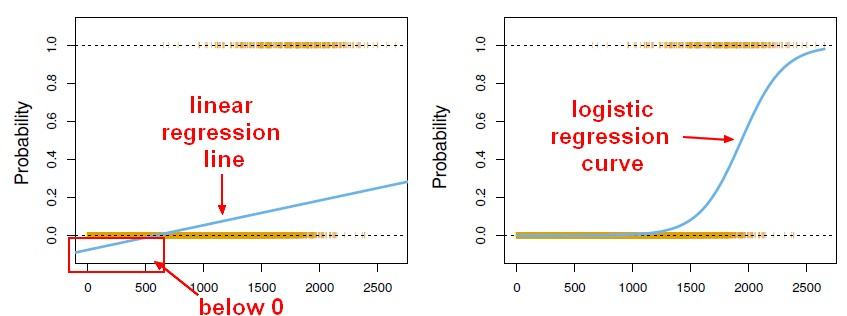
\includegraphics[scale=0.345]{pic/logistic_regression_vs_linear.jpg}
\note[item]{The linear regression model is based on an assumption that 
the outcome Y is continuous, with errors are normally distributed.}
\note[item]{if the outcome is binary, this is clearly violated}
\note[item]{Predicted values may be out of range, for 0,1, the linear
regression prediction will be out of this range}
\end{frame}

\begin{frame}
    \frametitle{Logistic Regression}

In logistic regression, the dependent variable is binary i.e. it only 
contains data coded as 1 (TRUE, success, positive, etc.) or 0 (FALSE, 
failure, negative, etc.)

The goal of logistic regression is to find:

\begin{itemize}
\item best fitting  model to describe the relationship between the 
binary characteristic of interest and a set of independent variables. 
\end{itemize}

\end{frame}


\begin{frame}
    \frametitle{Logistic Regression}
Logistic regression generates the coefficients (and its standard 
errors and significance levels) of a formula to predict a logit 
transformation of the probability of presence of the characteristic 
of interest:
 
 \begin{equation}
	logit(p)=\beta_0+\beta_1 x_1+\beta_2 x_2 +\ldots+\beta_k x_k
\end{equation}
where p is the probability of presence of the characteristic of 
interest.

\end{frame}

\begin{frame}
    \frametitle{Logistic Regression}
  The logit transformation is defined as the logged odds:
  
\begin{equation}
	Odds = \frac{p}{1-p} = \frac{\text{Prob of yes}}
    {\text{Prob of no}}
\end{equation}

And 
\begin{equation}
logit(p) = \ln{\frac{p}{1-p}}
\end{equation}
\end{frame}



\begin{frame}
\frametitle{Logistic Regression: Variables}

\begin{enumerate}
\item Academic: HS GPA, ACT/SAT, HS Percentile.
\item Financial: Pell Grant, EFC, Out-of-pocket, Scholarship,
	Unemployment rate.
\item Demographic: High School, Tier, Ethnicity. 
    \note[item]{The variables collection is rather limited compared
    to some of the studies}
\end{enumerate}

\end{frame}



\begin{frame}
\frametitle{Logistic Regression: Results}
\begin{table}[H]
\centering
 \tiny
 \setlength\tabcolsep{3pt}
    \begin{tabular}{|c|c|c|c|c|c|c|c|c|c|c|c|}
    \hline \hline
    \multicolumn{12}{ |c| }{GPA 2.9, ACT 19 }  \\ \hline
& Student               & 0       & 1000    & 2000    & 3000    & 4000    &5000    & 6000    & 7000    & 8000    & 10000   \\ \hline
1& 2.9-Tier1-19-White    & 59.55 & 64.63 & 69.39 & 73.77 & 77.73 & 81.24 & 84.31 & 86.96 & 89.22 & 91.72 \\ \hline
2& 2.9-Tier5-19-White    & 36.96 & 40.20 & 43.53 & 46.92 & 50.34 & 53.75 & 57.13 & 60.45 & 63.67 & 69.74 \\ \hline
     \multicolumn{12}{ |c| }{GPA 3.3, ACT  25 }   \\ \hline
3& 3.3-Tier1-25-Hispanic & 23.80 & 27.44 & 31.42 & 35.69 & 40.20 & 44.88 & 49.65 & 54.43 & 59.13 & 67.97 \\ \hline
4& 3.3-Tier1-25-White    & 55.60 & 59.32 & 62.94 & 66.42 & 69.72 & 72.84 &75.75 & 78.43 & 80.90 & 85.17 \\ \hline
    \multicolumn{12}{ |c| }{GPA 3.8, ACT 28 }     \\ \hline
5& 3.8-Tier1-28-White    & 42.29 & 46.05 & 49.85 & 53.65 & 57.41 & 61.08 &64.63 & 68.03 & 71.25 & 77.07 \\ \hline
6& 3.8-Tier4-28-White    & 20.54 & 22.87 & 25.37 & 28.05 & 30.89 & 33.89 &37.02 & 40.26 & 43.60 & 50.41 \\ \hline
    \end{tabular}
%  \caption{Prediction of enrollment under different levels of  
% scholarships}

\end{table}

The probability of enrollment increases with the increase of 
scholarship awards. Though these observations are not surprising, 
accurate  quantitative prediction of these probabilities is 
essential to the allocation of scholarship.
\end{frame}

\subsection{Number of Years Prediction}

\begin{frame}
\frametitle{Number of years prediction}
The following methods are compared to predict how long will a student stay in school:

\begin{table}[H]
\centering
\scriptsize
\label{num_year}
\begin{tabular}{|c|c|c|c|c|} \hline
    & \multicolumn{2}{c|}{10-Fold Cross Validation} &
\multicolumn{2}{c|}{Test Data} \\ \hline
Model                        & RMSE                  & MAE                   & RMSE           & MAE           \\ \hline
GLM                          & 1.40                  & 1.2                   & 1.53           & 1.26          \\ \hline
SVM(Linear Kernel)           & 1.44                  & 1.20                  & 1.62           & 1.32          \\ \hline
Decision Tree                         & 1.43                  & 1.24        & 1.43           & 1.23          \\ \hline
Stochastic Gradient Boosting & 1.40                  & 1.19                  & \textbf{1.40}           & \textbf{1.19}    \\ 
\hline
\end{tabular}
\end{table}
\note[item]{A gradient descent procedure is used to minimize the loss when adding trees. weaker learner to better learner}
\end{frame}


\subsection{Optimization Model}
\begin{frame}
\frametitle{Optimization Model}
The prediction of enrollment and graduation provide some 
insights of how students response to the various
scholarship. 

However, they have not addressed the allocation of limited
financial aid to students fundamentally.

% Questions like the following are addressed: 
% \begin{enumerate}
% \item Should we allocate the money to local students as they 
% are our bread and butter students and require less money?
% \item Should we allocate the money to 
% far-away students as local students will come anyway?
% \end{enumerate}  
\end{frame}


\begin{frame}
\frametitle{Math notation}
\textbf{Sets}:
\begin{itemize}
\item I:   set of applicants,  indexed by $i$ and $j$ \\
\item  M:  different levels of financial awards, indexed by 
$m$\\
$m \in  M = \{ 0,1000, 2000, \ldots ,8000\} $ \end{itemize}


\textbf{Variables}:
\begin{itemize}
\item $x_{im}$ :
whether a financial award $m$ 
is allocated to applicant $i$ or not
\end{itemize}

\end{frame}

\begin{frame}
\frametitle{Math notation}

\textbf{Parameters}:
\begin{itemize}
\item $p^e_{im}$: \hspace{0.3cm}  probability of enrollment for applicant 
$i$, if given award $m$
\item $p^g_{im}$: \hspace{0.3cm}  probability of graduation for applicant 
$i$, if given award $m$ 
\item $N_{im}$: \hspace{0.3cm}   expected number of years student $i$ 
stays at the institution, if given award $m$
\item $d(i,j)$: \hspace{0.3cm}    1 if applicant $i$ dominates 
applicant $j$; 0 otherwise.
\item B:      \hspace{0.3cm} total budget for financial aid
\item $A_m$:   \hspace{0.1cm} monetary value of award $m$
\item $T_i$:   \hspace{0.2cm} tuition paid by applicant $i$
\item $SSI_i$: \hspace{0cm} government compensation for
				applicant $i$ when he/she graduates

\end{itemize}
\end{frame}




\begin{frame}{fragile}
\frametitle{Objective}
\textbf{Maximize the total revenue}: tuition revenue + SSI 
income

\scriptsize{
 $\max \quad \sum_{i\in I} \sum_{m\in M} x_{im}\cdot p^e_{im}\cdot(T_i-A_m)\cdot N_{im}+
\sum_{i\in I} \sum_{m\in M} x_{im}\cdot p^e_{im} \cdot p^g_{im}\cdot SSI_i$

}


\end{frame}


\begin{frame}
\frametitle{Constraints}
\begin{enumerate}
\item Each student only get one scholarship: $\sum_{m \in 
M}x_{im}=1  \hspace{1cm} \forall i\in I $
\vfill
\item Total budget constraint: 

$\sum_{i \in I} \sum_{m\in M} 
x_{im}\cdot p^e_{im}\cdot A_m\leq B $
\vfill
\item Dominance constraint:

$ \sum_{m \in M} x_{im}\cdot A_m \geq \sum_{m \in M} 
x_{jm}\cdot A_m \hspace{1cm}  \forall
(i,j)|d(i,j)=1 $

\end{enumerate}
\end{frame}



\begin{frame}
\frametitle{Pair-wise Dominance Constraints}
More than 5,500 applicants each year.

For the dominance constraints:

There are $(5,500 \times 5,500) / 2$ or 
more than 15 million constraints.

\begin{table}[H]
\centering
\begin{tabular}{|c|c|c|}
\hline
  Applicant & GPA & ACT \\ [0.5ex] 
\hline
1 & 2.9 & 18 \\ \hline
2 & 3.7 & 21 \\ \hline
3 & 3.8 & 30 \\ \hline
4 & 2.7 & 21 \\ \hline
5 & 3.3 & 17 \\ \hline
6 & 3.9 & 27 \\ \hline
\end{tabular}
\end{table}

\end{frame}

\begin{frame}
\frametitle{Full and redundant dominance }

 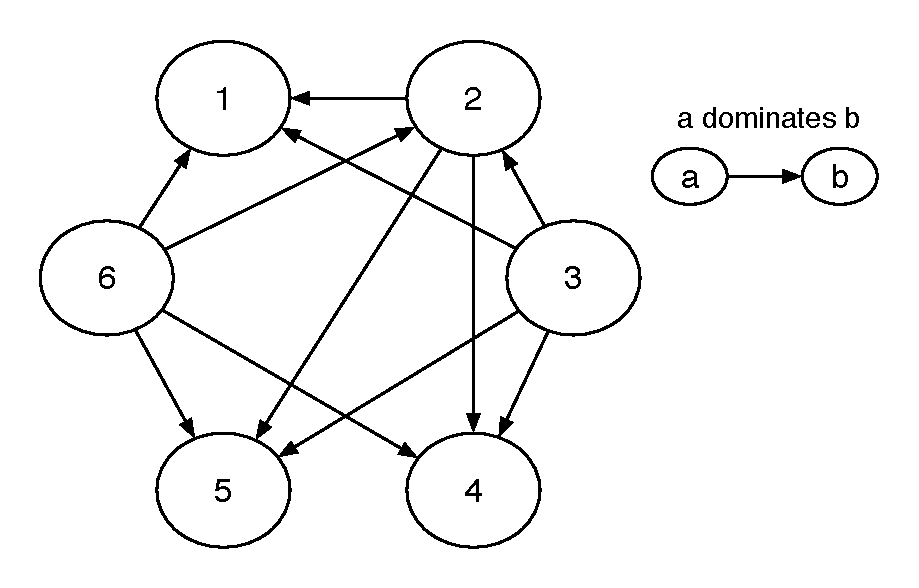
\includegraphics[scale=0.4]{pic/dominance1.eps}
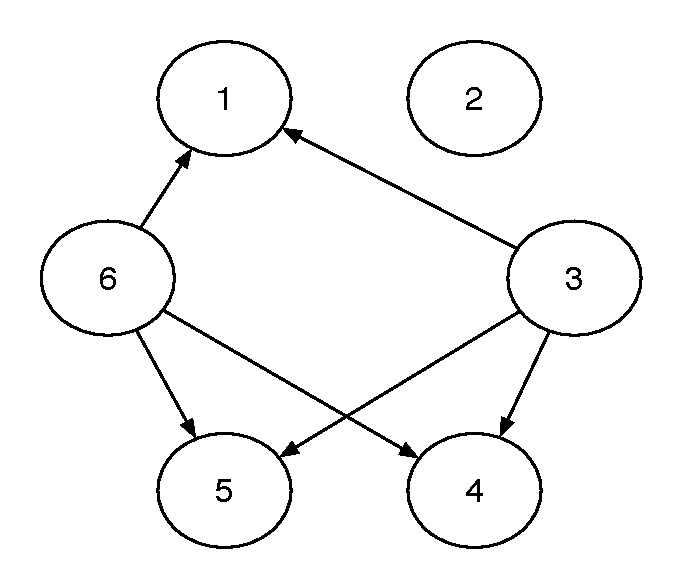
\includegraphics[scale = 0.4]{pic/dominance2.eps}
\end{frame}

\begin{frame}
\frametitle{Minimum dominance}
\begin{center}
 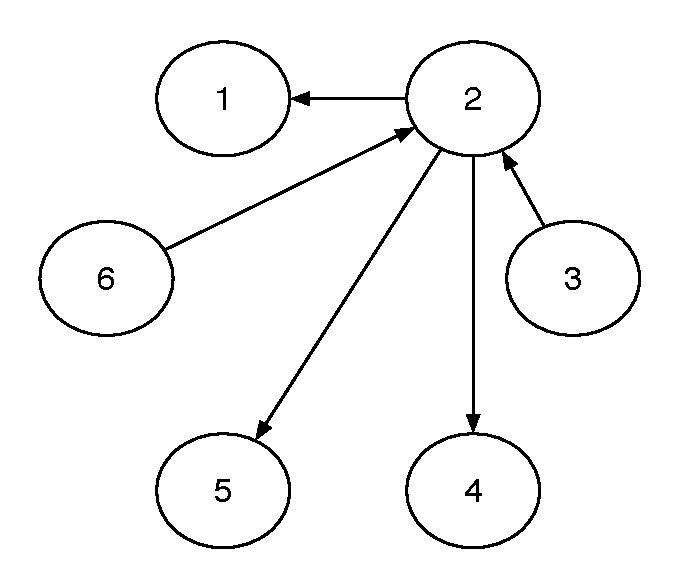
\includegraphics[scale = 0.4]{pic/dominance3.eps}
\end{center}
 
\begin{center}
 \begin{tabular}{l|llllll}
        & 1 & 2 & 3 & 4 & 5 & 6 \\ \hline
        1 & 0 & 0 & 0 & 0 & 0 & 0 \\
        2 & 1 & 0 & 0 & 1 & 1 & 0 \\
        3 & 0 & 1 & 0 & 0 & 0 & 0 \\
        4 & 0 & 0 & 0 & 0 & 0 & 0 \\
        5 & 0 & 0 & 0 & 0 & 0 & 0 \\
        6 & 0 & 1 & 0 & 0 & 0 & 0
    \end{tabular}
\end{center}
    
\end{frame}


\begin{frame}
\frametitle{Size of the optimization models}

\centering
\scriptsize{
\begin{tabular}{|c|l|c|c|}
\hline %\hline
\multicolumn{2}{|c|}{Model Components}   &
Original Model & Reduced Model \\ \hline
Variables                   & \multicolumn{1}{|l|}{Allocation (binary) 
$x_i$}
& 57,860         & 57,860        \\ \hline
\multirow{3}{*}{Constraint} & One Award per ID         &
5,260          & 5,260         \\ \cline{2-4}
& Dominance                & 13,833,800     & 191,497
\\ \cline{2-4}
& Total Budget              & 1              & 1
\\ \cline{2-4}
& Total Number of Constraints     & 13,839,061     & 196,758
\\ \hline
\end{tabular}
}


\end{frame}


\frametitle{Results}
\begin{frame}
\begin{figure}
    \centering
  \includegraphics[width=8cm, height=6cm,scale=0.2]{pic/ssi_10k.eps}
\end{figure}
\end{frame}


\begin{frame}
\frametitle{Results}
\begin{figure}
    \centering
  \includegraphics[width=8cm, height=6cm,scale=0.2]{pic/ssi_12k.eps}
\end{figure}
\end{frame}


\begin{frame}
\frametitle{Results}
\begin{figure}
    \centering
  \includegraphics[width=8cm, height=6cm,scale=0.2]{pic/ssi_14k.eps}
\end{figure}
\end{frame}

\subsection{Implementation}

\begin{frame}
\frametitle{Implementation and Policy}
\begin{itemize}
\item The scholarship allocation of individual 
student and optimal budget are solved above.
\item However, the enrollment administration need a 
simpler policy to implement.
\item  Decision tree and piece-wise linear regression were used for this task.
\end{itemize}
 
\end{frame}

\begin{frame}
\frametitle{Decision tree policy}
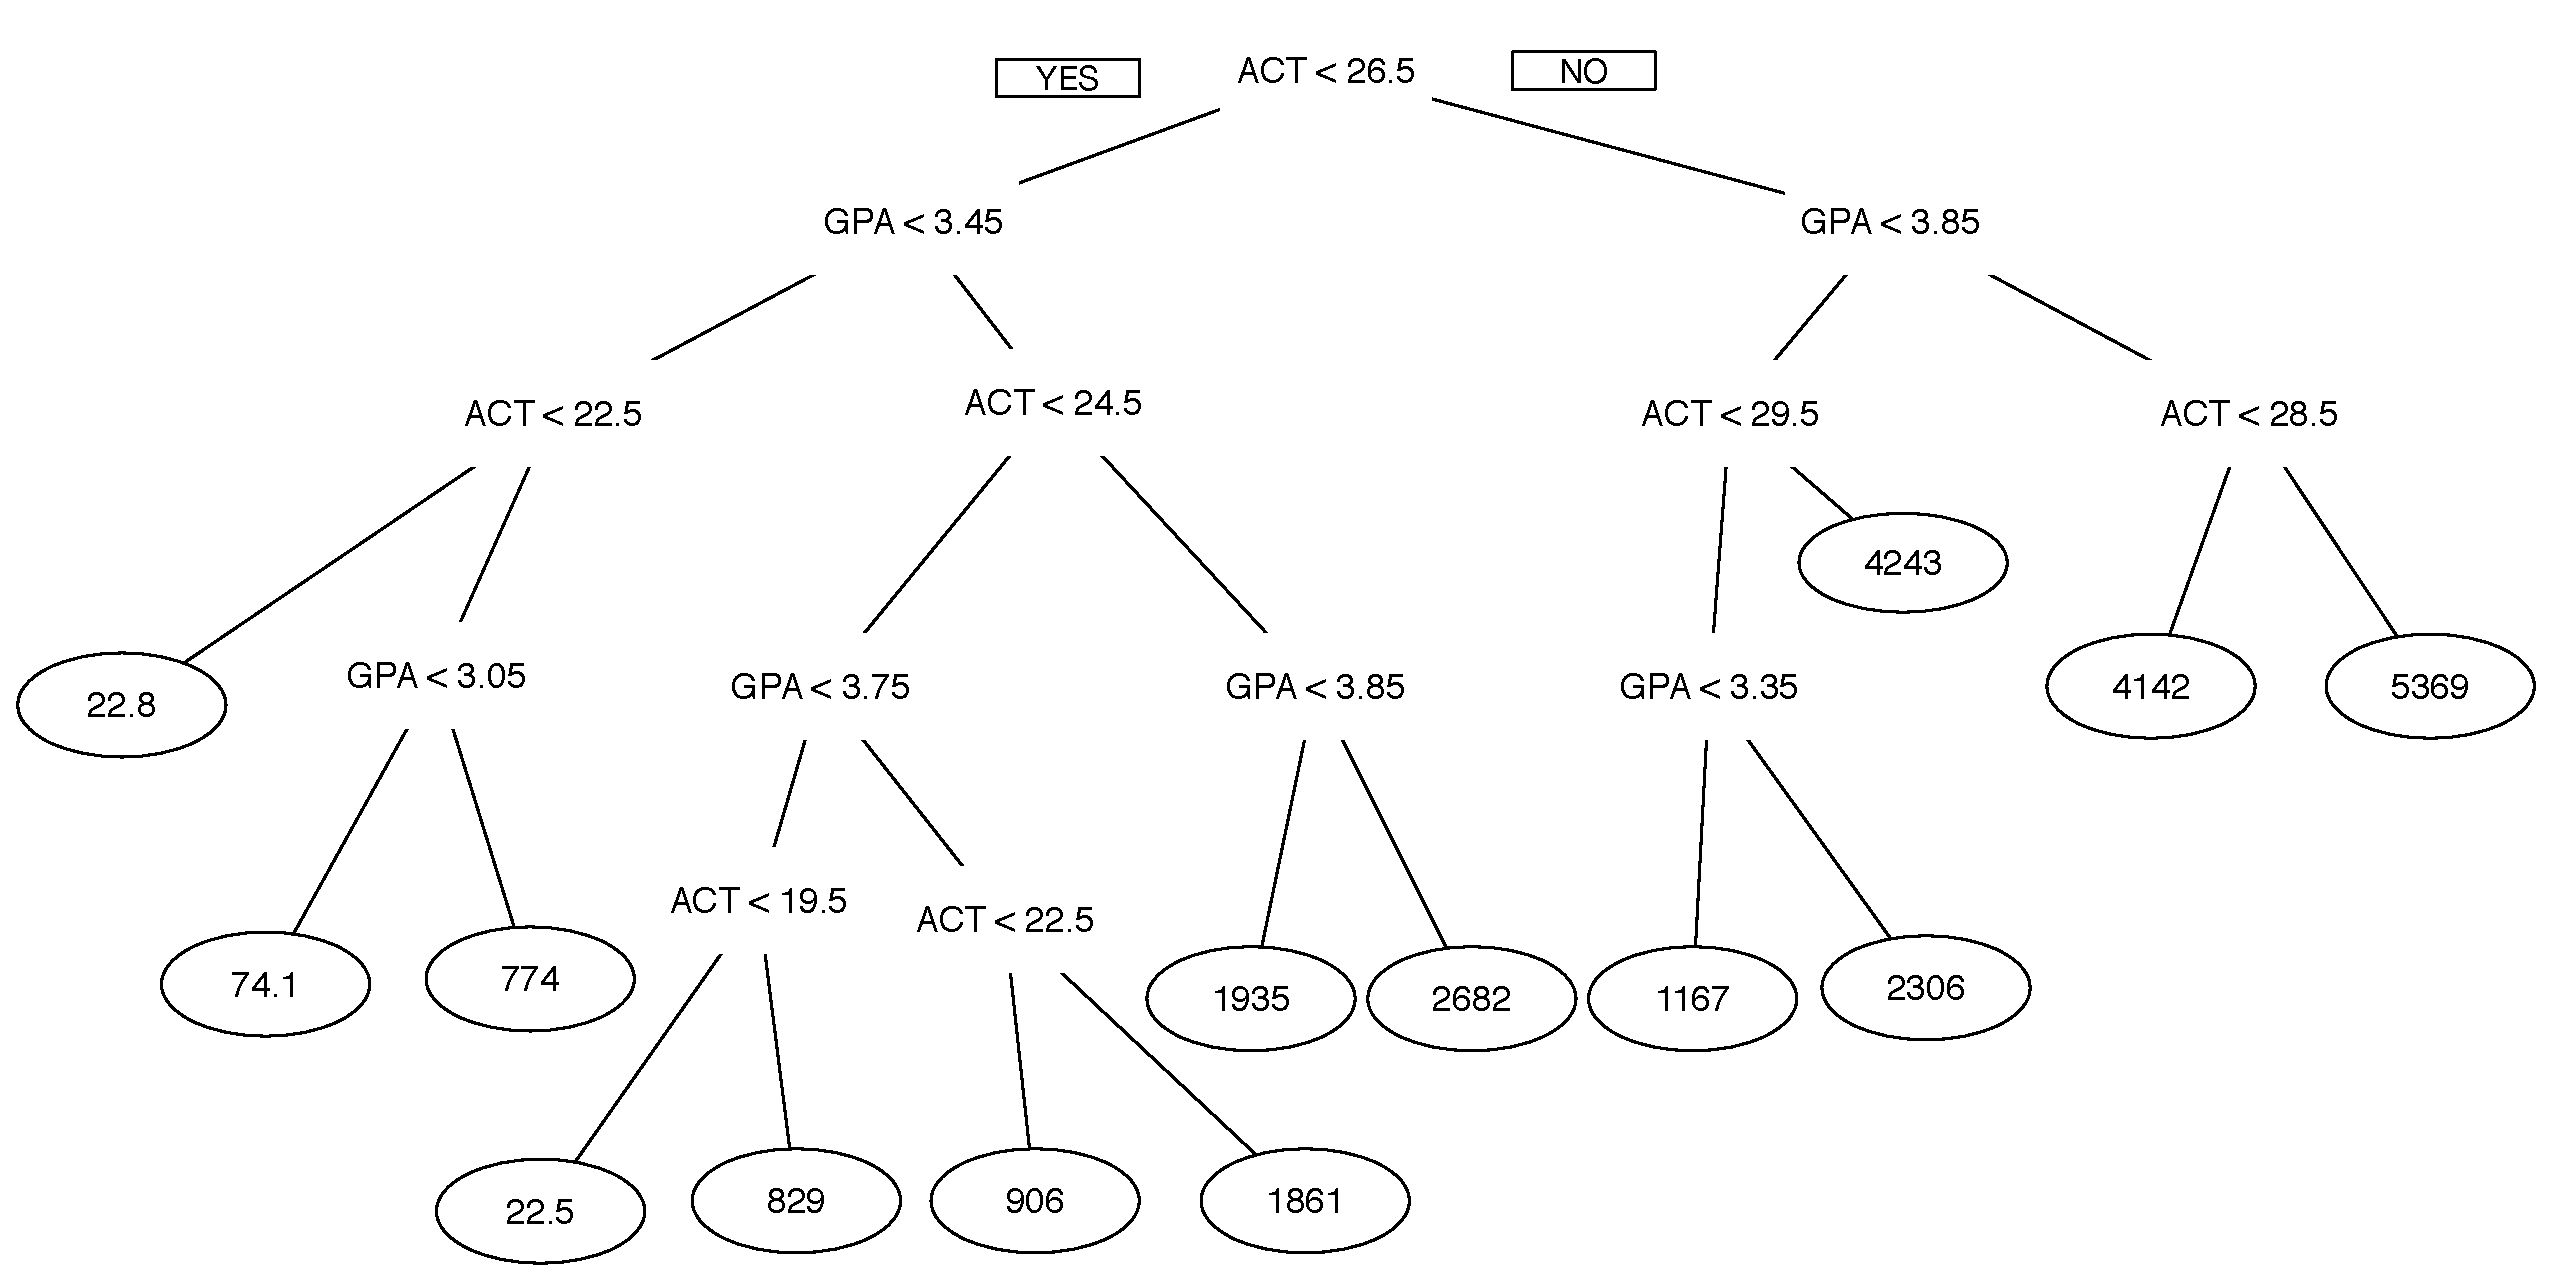
\includegraphics[width=10cm, height=6cm, scale = 0.4]
{pic/FA_DT_Result.eps}
\end{frame}


\begin{frame}
\frametitle{Piece-wise linear regression results}
Simplified version of policy in piece-regression form.
\begin{table}[H]
\centering
\begin{tabular}{|c|c|} \hline
Composite Score & Scholarship Amount \\ \hline
0-54.9         & 0              \\ \hline
55-59.9         & 1,500              \\ \hline
60-65.9         & 2,500              \\ \hline
66-69.9         & 3,500              \\ \hline
70-74.9         & 4,500              \\ \hline
75+             & 6,000              \\ \hline
\end{tabular}
\end{table}
\end{frame}


\begin{frame}
\frametitle{Business impact and Application}
\begin{itemize}
\item  The result of the study has been successfully implemented in the 
state university and has resulted in millions of financial benefits. 
\item The research would be applicable to many other institutions and offers 
a methodology, tools and insights into the solution of financial aid 
problems. 
\end{itemize}

\end{frame}


\subsection{Summary}
\begin{frame}
\frametitle{Summary}
\begin{enumerate}
\item A serious of models are developed to predict:
  \begin{itemize}
    \item Enrollment probability
    \item Graduation probability
    \item Number of years of stay
  \end{itemize}
\item Developed minimum cardinality dominance table to reduce the model size. 
\item An optimization model is developed with the objective to maximize the revenue.
\item A regression analysis is developed to translate the optimization results to
	managerial insights and derive a policy for implementation.
\end{enumerate}
\end{frame}


\subsection{Limitation}
\begin{frame}
\frametitle{Limitation}
\begin{itemize}
\item The prediction of student's enrollment decision is 
hard.
\item The research is also limited by the availability of 
data provided by the institution under study.
\end{itemize}

\note[item]{is by itself a hard problem, because 
enrollment in a particular institution is determined by 
many factors that are not available to the institution.
For example, it is well known that the students' decision  is affected by family influence and other factors, which are not traceable or measurable.}

\end{frame}

\subsection{Future Study}
\begin{frame}
\frametitle{Future Study}
The results from the optimization specify the scholarship awards to each applicant under a 
specific population and budget.  
\begin{itemize}
\item  The actual size and composition of the application pool could be affected by the 
       unemployment rate and is random in nature. 
\item  Stochastic optimization techniques such as sampling to find the optimal allocation 
under a random pool will be of great interest. 

\end{itemize}

\note[item]{Nevertheless, at this stage, this study is on optimization under a specific pool}
\end{frame}




\section{Acknowledgement}
\begin{frame}
    \frametitle{Thank you!}
    Dissertation Committee:
    \begin{itemize}
    \item Dr. Xinhui Zhang
    \item Dr. Pratik Parikh
    \item Dr. Caroline Cao
    \item Dr. Subhashini Ganapathy
    \item Dr. Nan Kong
    \end{itemize}
    \note{ I would like to express my sincere gratitude to my advisor DR. Zhang for the continuous support of my study.
    Thank you for your patience, motivation and knowledge.}
    \note{Besides my advisor, I would like to thank the rest of my thesis committeei DR......  for serving as my committee.
    I want to thank you for letting my defense be an enjoyable moment, and thank you for the valuable comments and suggestions, thanks to 
    you.}
\end{frame}


\begin{frame}
\frametitle{}
\end{frame}


\begin{frame}
\frametitle{}
\end{frame}


\begin{frame}
\frametitle{}
\end{frame}


\begin{frame}
\frametitle{}
\end{frame}



\begin{frame}
\frametitle{}
\end{frame}







\bibliographystyle{plainnat}
\bibliography{shuai_cita}
\end{document}


